\documentclass{jsarticle}
\usepackage{bm}
\usepackage{amsmath}
\usepackage{listings, jlisting}
\usepackage{}
\usepackage[dvipdfmx]{graphicx}
\usepackage[hang,small,bf]{caption}
\usepackage[subrefformat=parens]{subcaption}
\captionsetup{compatibility=false}

\lstset{
  basicstyle={\ttfamily},
  identifierstyle={\small},
  commentstyle={\smallitshape},
  keywordstyle={\small\bfseries},
  ndkeywordstyle={\small},
  stringstyle={\small\ttfamily},
  frame={tb},
  breaklines=true,
  columns=[l]{fullflexible},
  numbers=left,
  xrightmargin=0zw,
  xleftmargin=3zw,
  numberstyle={\scriptsize},
  stepnumber=1,
  numbersep=1zw,
  lineskip=-0.5ex
}
\renewcommand{\lstlistingname}{プログラム}

\title{信号処理II フルレポート(1)}
\author{2022531047 \\中山 涼太}
\begin{document}
\maketitle \newpage

\section*{課題1}
\begin{quote}
    重み付き最小自乗法による最適なフィルタ係数の導出式を求めよ。\\
\end{quote}
最小自乗法は自乗誤差が最小となるパラメータを求める問題であり、
式(\ref{original_lsm})で表される計算で処理される。
\begin{equation} \label{original_lsm}
    \min_a E = \int_{-\pi}^{\pi} |W(\omega)(H(\omega)-D(\omega))|^2
\end{equation}
\begin{align*}
    H(\omega) &= a_0 + a_1 e^{-j\omega} + a_2 e^{j2\omega} + \cdots + a_N e^{-jN\omega}\\
    D(\omega) &\text{:所望周波数特性}\\
    W(\omega) &\text{:重み関数}\\
    E&\text{:評価関数}
\end{align*}
ここで、$H(\omega_k)$を次のように行列表現する。
\begin{align*}
    \bm{a} &=
    \begin{bmatrix}
        a_0\quad a_1\quad \cdots \quad a_N
    \end{bmatrix}^t\\
    \bm{q_k} &= \begin{bmatrix}
        1\quad e^{j\omega_k}\quad e^{j2\omega_k}\quad \cdots e^{jN\omega_k}
    \end{bmatrix}^t\\
    H(\omega_k) &= \bm{q_k}{}^t \bm{a}
\end{align*}
$\bm{a}$はフィルタ係数を並べたベクトル、$\bm{q_k}$は周波数点$\omega_k$の値を並べたベクトルである。
さらに$\bm{q_k}$を並べたベクトルを$\bm{Q}$とすると、

式(\ref{original_lsm})を次のように行列表現する。
\begin{equation}
    E'' = \sum_{k=0}^{L-1}|W(\omega_k) (H(\omega_k) - D(\omega_k))|^2
\end{equation}
ここで、$\bm{W}=\text{diag}{W(\omega_k)}, \quad \bm{E} = \bm{W(Qa-d)}$より、
\begin{equation}
    E''=(\bm{Qa}-\bm{d})^t \bm{W}^t \bm{W} (\bm{Qa}-\bm{d})
\end{equation}
ここで、$\bm{W}=\text{diag}{W(\omega_k)}$は対角行列のため、$\bm{W}=\bm{W}^t$である。したがって、
\begin{align}
    E''&=(\bm{Qa}-\bm{d})^t \bm{W}^2 (\bm{Qa}-\bm{d})\\
    &=\bm{a}^t \bm{Q}^t \bm{W}^2 \bm{Qa} -2\bm{a}^t \bm{Q}^t \bm{W}^2 \bm{d} + \bm{d}^t \bm{W}^2 \bm{d}
\end{align}
と整理できる。$\bm{Q}^t \bm{W}^2 \bm{Q}$が常に対称行列であることより、評価関数を$\bm{a}$で偏微分すると、次の式が得られる。
\begin{equation}
    \frac{\partial E''}{\partial \bm{a}} =
    \begin{bmatrix}
        \frac{\partial E''(\bm{a})}{\partial a_0}\quad \frac{\partial E''(\bm{a})}{\partial a_1\quad}\quad \cdots \frac{\partial E''(\bm{a})}{\partial a_N}
    \end{bmatrix}^t
     = 2\bm{Q}^t \bm{W}^2 \bm{Qa} - 2\bm{Q}^t \bm{W}^2 \bm{d}
\end{equation}
これが0となる$\bm{a}$が最小自乗解であるので、
\begin{align}
    2\bm{Q}^t \bm{W}^2 \bm{Qa} - 2\bm{Q}^t \bm{W}^2 \bm{d} = 0\\
    \bm{Q}^t \bm{W}^2 \bm{Qa} - \bm{Q}^t \bm{W}^2 \bm{d} = 0\\
    (\bm{Q}^t \bm{W}^2 \bm{Q})^{-1} \bm{Q}^t \bm{W}^2 \bm{Qa} = (\bm{Q}^t \bm{W}^2 \bm{Q})^{-1} \bm{Q}^t \bm{W}^2 \bm{d}\\
    \bm{a} = (\bm{Q}^t \bm{W}^2 \bm{Q})^{-1} \bm{Q}^t \bm{W}^2 \bm{d}
\end{align}
と$\bm{a}$が求められる。

\section*{課題2}
\begin{quote}
    重み付き最小自乗法によるローパスフィルタの設計プログラムを完成させよ。
\end{quote}
課題1で導出した$\bm{a}$を用いたローパスフィルタのプログラムが以下のプログラム\ref{wlsm}である。

\begin{lstlisting}[caption={重み付き最小自乗法を用いたローパスフィルタ}, label={wlsm}]
clear all; clc; close all

N=24;   % フィルタ係数の数(フィルタ長2N-2)
L=1024; % 周波数サンプル数
dw = pi/(L-1);
wp = 0.25;  % 通過域のエッジ
ws = 0.29;  % 阻止域のエッジ

pe = ceil(wp*L);
se = ceil(ws*L);

d = [ones(pe, 1); zeros(L-pe, 1)];  % 所望特性
Q = [ones(L, 1) cos((0:L-1)'*(1:(N-1))*dw)];    % 規定周波数成分を並べた行列

pm = 0.1;   % 通過域の重み
sm = 1.0;   % 阻止域の重み
w = [pm*ones(pe, 1); zeros(se - pe, 1); sm*ones(L - se, 1)]; % 重みベクトル
W = diag(w);    % 重みベクトルを対角成分に持つ対角行列

a = (Q'*W^2*Q)\(Q'*W^2*d);  % 重み付き最小自乗法によるフィルタ係数の推定

coef = [flipud(a(2:end))/2; a(1); a(2:end)/2];  % フィルタ係数の対称性により、長さ2N-2のフィルタ係数を導出

H = fft(coef, 2*L); % 設計したフィルタの周波数特性H
figure(1); plot(1:length(H(1:L)), abs(H(1:L)), 1:length(H(1:L)), d)
\end{lstlisting}
\newpage
\section*{課題3}
\begin{quote}
    最小自乗法によるローパスフィルタと、重み付き最小自乗法によるローパスフィルタの結果を比較し、その違いについて報告せよ。また、なぜ設計結果に違いが生じるのか考察せよ。
    ただし、各フィルタは下記の設定で設計すること。
    \begin{itemize}
        \item フィルタ係数の数:$N=24$
        \item 周波数サンプル数:$L=1024$
        \item 通過域のエッジ:$\omega_p=0.25\pi$
        \item 阻止域のエッジ:$\omega_s=\{0.29\pi, 0.32\pi, 0.35\pi\}$
    \end{itemize}
    重み付き最小自乗法による設計のみ、阻止域のエッジを変えたときの結果も報告すること。
\end{quote}
与えられた条件で
\begin{figure}[htbp]
    \centering
    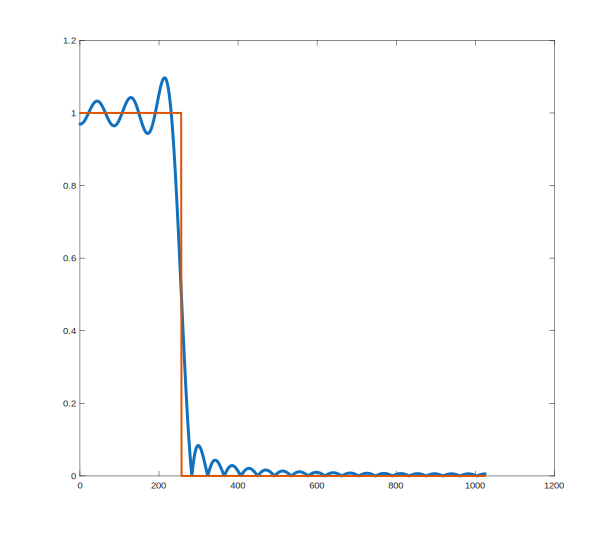
\includegraphics[width=5cm]{../img_7_24_0.25.png}
    \caption{最小自乗法によるローパスフィルタ}
\end{figure}
\begin{figure}[h]
    \begin{minipage}[htbp]{0.33\columnwidth}
        \centering
        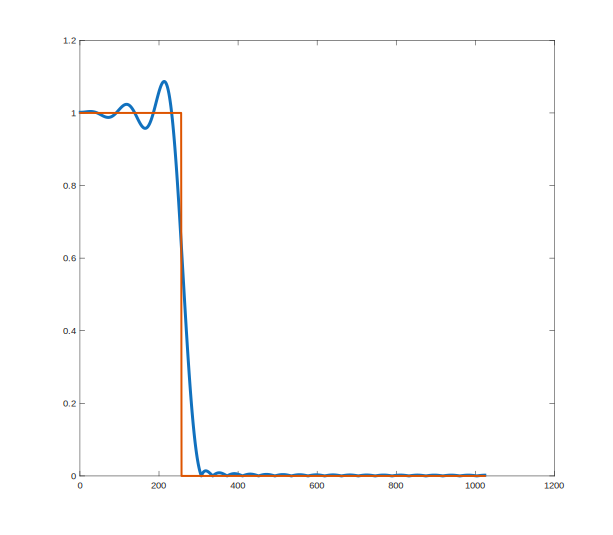
\includegraphics[width=0.98\columnwidth]{img_report_lp_0.29_0.1_1.png}
        \subcaption{$\omega_s = 0.29$}
    \end{minipage}
    \begin{minipage}[htbp]{0.33\columnwidth}
        \centering
        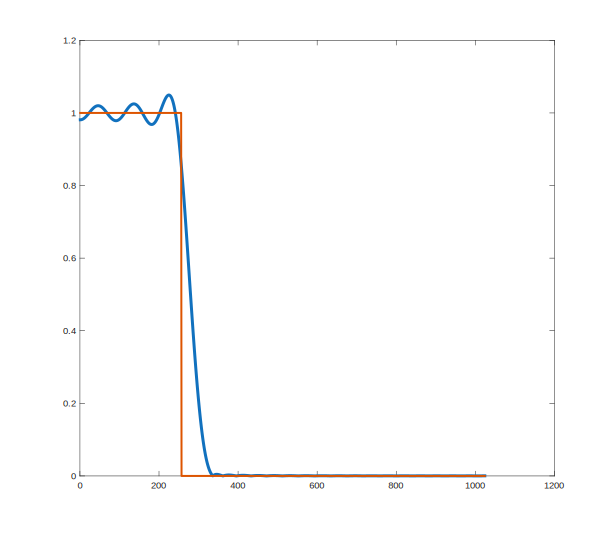
\includegraphics[width=0.98\columnwidth]{img_report_lp_0.32_0.1_1.png}
        \subcaption{$\omega_s = 0.32$}
    \end{minipage}
    \begin{minipage}[htbp]{0.33\columnwidth}
        \centering
        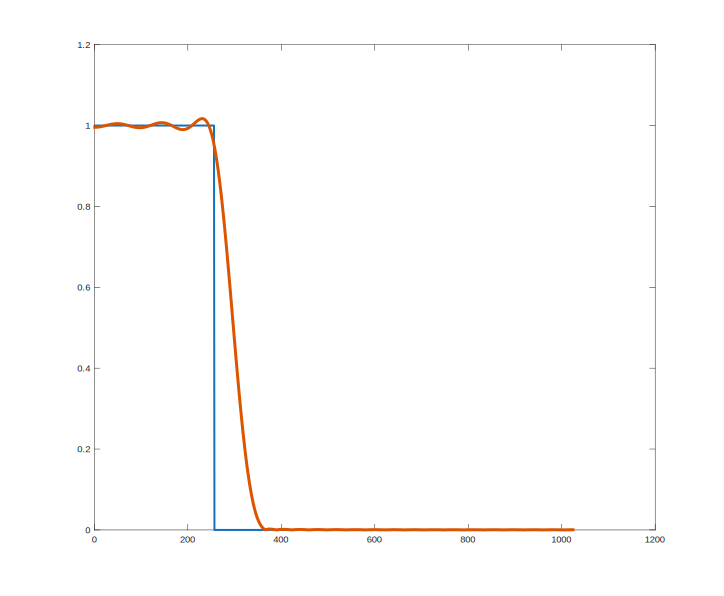
\includegraphics[width=0.98\columnwidth]{img_report_lp_0.35_0.1_1.png}
        \subcaption{$\omega_s = 0.35$}
    \end{minipage}
    \caption{重み付き最小自乗法によるローパスフィルタ\\$\alpha = 0.1, \beta = 1.0$}
\end{figure}

\section*{課題4}

\end{document}